%! BibTeX Compiler = biber
%TC:ignore
\documentclass{article}

\usepackage{xcolor, colortbl}
\definecolor{BLUELINK}{HTML}{0645AD}
\definecolor{DARKBLUELINK}{HTML}{0B0080}
\PassOptionsToPackage{hyphens}{url}
\usepackage[colorlinks=false]{hyperref}
% for linking between references, figures, TOC, etc in the pdf document
\hypersetup{colorlinks,
    linkcolor=DARKBLUELINK,
    anchorcolor=DARKBLUELINK,
    citecolor=DARKBLUELINK,
    filecolor=DARKBLUELINK,
    menucolor=DARKBLUELINK,
    urlcolor=BLUELINK
} % Color citation links in purple
\PassOptionsToPackage{unicode}{hyperref}
\PassOptionsToPackage{naturalnames}{hyperref}

\usepackage{biorxiv}
\usepackage[backend=biber,,isbn=false,url=false,intitle=true,style=nature]{biblatex}
\addbibresource{codon_models.bib}

\usepackage{url}
\usepackage{amssymb,amsfonts,amsmath,amsthm,mathtools}
\usepackage{lmodern}
\usepackage{xfrac, nicefrac}
\usepackage{bm}
\usepackage{listings, enumerate, enumitem}
\usepackage[export]{adjustbox}
\usepackage{graphicx}
\usepackage{bbold}
\usepackage{pdfpages}
\pdfinclusioncopyfonts=1
\usepackage{lineno}

\newcommand{\NS}[1]{\textcolor{red}{\textbf{\emph{[NS: #1]}}}}

\newcommand{\UniDimArray}[1]{\bm{#1}}
\newcommand{\BiDimArray}[1]{\bm{#1}}
\DeclareMathOperator{\E}{\mathbb{E}}
\DeclareMathOperator{\Var}{\textrm{Var}}
\newcommand{\der}{\textrm{d}}
\newcommand{\e}{\textrm{e}}
\newcommand{\avg}[1]{\left< #1 \right>} % for average
\newcommand{\Ne}{N_{\textrm{e}}}
\newcommand{\proba}{\mathbb{P}}
\newcommand{\pfix}{\proba_{\textrm{fix}}}
\newcommand{\dn}{d_N}
\newcommand{\ds}{d_S}
\newcommand{\dnds}{\dn / \ds}
\newcommand{\Sphy}{S}
\newcommand{\Sphyclass}{\mathcal{C}}
\newcommand{\SphyMean}{\overline{\Sphy}}
\newcommand{\divStrongDel}{\Sphy < -3}
\newcommand{\divDel}{-3 < \Sphy < -1}
\newcommand{\divWeakDel}{-1 < \Sphy < 0}
\newcommand{\divWeakAdv}{0 < \Sphy < 1}
\newcommand{\divAdv}{ \Sphy > 1}
\newcommand{\PdivStrongDel}{\proba \left[ \divStrongDel \right]}
\newcommand{\PdivDel}{\proba \left[ \divDel \right]}
\newcommand{\PdivWeakDel}{\proba \left[ \divWeakDel \right]}
\newcommand{\PdivWeakAdv}{\proba \left[ \divWeakAdv \right]}
\newcommand{\PdivAdv}{\proba \left[ \divAdv \right]}

\newcommand{\Spop}{\beta}
\newcommand{\SpopMean}{\overline{\Spop}}
\newcommand{\polyDel}{\Spop < -1}
\newcommand{\polyNeutral}{-1 < \Spop < 1}
\newcommand{\polyAdv}{ \Spop > 1}
\newcommand{\PpolyDel}{\proba \left[ \polyDel \right]}
\newcommand{\PpolyNeutral}{\proba \left[ \polyNeutral \right]}
\newcommand{\PpolyAdv}{\proba \left[ \polyAdv \right]}

\renewcommand{\baselinestretch}{1.5}
\linenumbers

\title{In mammals, 20 to 40\% of advantageous mutations are restoring damaged genomes instead of creating adaptive innovations}

\author{
    \large
    \textbf{T. {Latrille}$^{1}$, J. {Joseph}$^{2}$, N. {Salamin}$^{1}$}\\
    \normalsize
    $^{1}$Université de Lausanne, Lausanne, Switzerland\\
    $^{2}$Université de Lyon, CNRS, LBBE UMR 5558, Villeurbanne, France \\
    \texttt{\href{mailto:thibault.latrille@ens-lyon.org}{thibault.latrille@ens-lyon.org}} \\
}

\begin{document}
    \maketitle

    \begin{abstract}
        Positive selection can be the result of adaptive evolution, driven by a change in environment or selective pressure.
        However, positive selection can also be the result of what we call maintenance positive selection where advantageous mutations are compensating for deleterious substitutions without any change of the environment.
        The evolutionary outcomes of these two positive selections are drastically different.
        While adaptive evolution acts as a diversifying force, maintenance positive selection stabilizes phenotypes and reduces diversity across species.
        By leveraging polymorphism data in 28 populations and divergence data between 94 mammalian species, we estimate that 20 to 40\% of all new advantageous mutations are under maintenance positive selection.
        Our work confirms that deleterious substitutions have accumulated in mammals and are currently being compensated for, resulting in widespread positive selection that is not adaptive evolution.
    \end{abstract}

    \keywords{Selection \and phylogenetic \and population genetics \and codon models \and adaptation }

    %\NS{on devrait plus placer le départ de l'intro dans un contexte historique, pour dire que de connaître si une mutation est avantageuse est la base de la génétique moléculaire (en citant des papiers clés)}
    We usually say that a mutation is undergoing positive selection when it brings a fitness advantage to its bearer with the consequence of facilitating its own transmission to the next generation.
    We can distinguish two main scenarios that can lead to such positive selection.
    In the first scenario, a mutation towards a state which was deleterious is now advantageous because of a change of environment.
    A change of environment could be a change of temperature, viral exposition but it could also be a change in another part of the species' genome.
    In the new environment, the mutation allows its bearer to survive and reproduce more than the others and thus will be positively selected.
    This process is typically referred to as adaptive evolution (fig.~\ref{fig:fitness-landscape}A).

    The second scenario involves a mutation restoring the ancestral allele which corresponded to an optimal fitness for an individual in a constant environment, but has been lost due to the fixation of a deleterious mutation by drift (fig.~\ref{fig:fitness-landscape}B).
    In this study, this process will be referred to as maintenance positive selection.
    At the scale of a population, these two scenarios display different dynamics.
    While in the case of environmental change, the population as a whole is climbing the fitness landscape along an adaptive walk\cite{tenaillon_utility_2014}, in the case of maintenance positive selection, the population as a whole is at mutation-selection equilibrium and therefore merely stays at the same location in the fitness landscape\cite{sella_application_2005, mustonen_fitness_2009}.

    At the population scale, these two different kinds of selection are indistinguishable and both result in a positive transmission bias of the advantageous allele, but their consequences at a macro-evolutionary scale are fundamentally different.
    While adaptive evolution promotes phenotype diversification (fig.~\ref{fig:fitness-landscape}C), maintenance positive selection promotes phenotype stability and preserves well established biological systems (fig.~\ref{fig:fitness-landscape}D).
    It is thus essential to distinguish these two types of positive selection to understand the long term effects of selection on the diversification of species.

    Positive selection can be quantified by comparing sequence variation inside a population with the sequence divergence from a sister species\cite{mcdonald_adaptative_1991}.
    The basic idea is that advantageous mutations are expected to be observed in substitutions between species but not in polymorphism within a population because they reach fixation too quickly.
    This method has been largely improved to account for possible bias-inducing factors such as the presence of weak positive selection, background selection and demographic fluctuations\cite{eyre-walker_distribution_2006, eyre-walker_estimating_2009, galtier_adaptive_2016, tataru_inference_2017}.
    It has been applied across many organisms and enabled the discovery of widespread positive selection\cite{moutinho_variation_2019}.
    However, the exact causes for this widespread occurrence of positive selection have been scarcely investigated\cite{eyre-walker_distribution_2006, eyre-walker_estimating_2009, galtier_adaptive_2016} %\NS{is it the case in the conclusion of the previous paper?? would be nice to back it up with references}.
    As mentioned above, not all advantageous mutations contribute to genetic innovation and diversification and truly adaptive evolution can only be well estimated if maintenance positive selection is taken into account.
    While adaptive evolution is unpredictable because it caused by an unpredictable change in the environment of organisms, the second is predictable because optimal states should be more or less the same for closely related organisms which share most of their environment and physiology.
    A way to thus measure maintenance positive selection is to predict selection coefficients assuming a constant and stable fitness landscape estimated from the alignment of protein-coding genes.
    For each site of the protein alignment, a first approximation would be to consider that the frequency of an amino-acid is a proxy for its fitness, since for example a deleterious amino acid will be more likely to be absent in the alignment.
    One of the most used methods to make these predictions is SIFT (Sort Intolerant From Tolerant), which reliably detects deleterious mutations in many taxa\cite{ng_sift_2003, vaser_sift_2016}.
    However, this method has two major shortcomings.
    First, we know that a lot of mechanisms can influence amino-acid frequency other than fitness (phylogeny, mutation biases, GC-biased gene conversion, mutational paths) which are not accounted for in SIFT.
    Second, SIFT scores makes little sense as an actual measure of fitness, and is not interpretable in terms of population genetics.
    Contrarily, so-called mutation-selection codon models are rooted within a population genetics formalism\cite{halpern_evolutionary_1998, mccandlish_modeling_2014}.
    These phylogenetic codon models can disentangle processes of mutation at the DNA level and selection at the amino-acid level.
    Such codon models provide a nearly-neutral framework of evolution by estimating the fitness landscape over amino-acid sequences for each site of the sequence (fig~\ref{fig:method}A) while taking into account non-adaptive processes impacting codon frequency\cite{halpern_evolutionary_1998, rodrigue_mechanistic_2010, tamuri_estimating_2012}.
    %Only nearly-neutral mutations between high fitness amino acids will tend to be permitted by the model, allowing for the explicit calculation of the scaled selection coefficient of non-synonymous mutations between codons.
    As a consequence, by integrating datasets at the species and population level, we can estimate the selection coefficient for each mutation currently segregating in a population.
    Such a dataset can allow us to address different questions regarding positive selection affecting protein-coding DNA sequences.
    Which proportion of the segregating polymorphisms are predicted to be positively selected, from a suboptimal to a more optimal amino acid?
    Are these polymorphisms actually under ongoing positive selection at the scale of populations?
    Finally, how much of the recent substitutions are due to maintenance positive selection?

    \begin{figure*}[!ht]
        \centering
        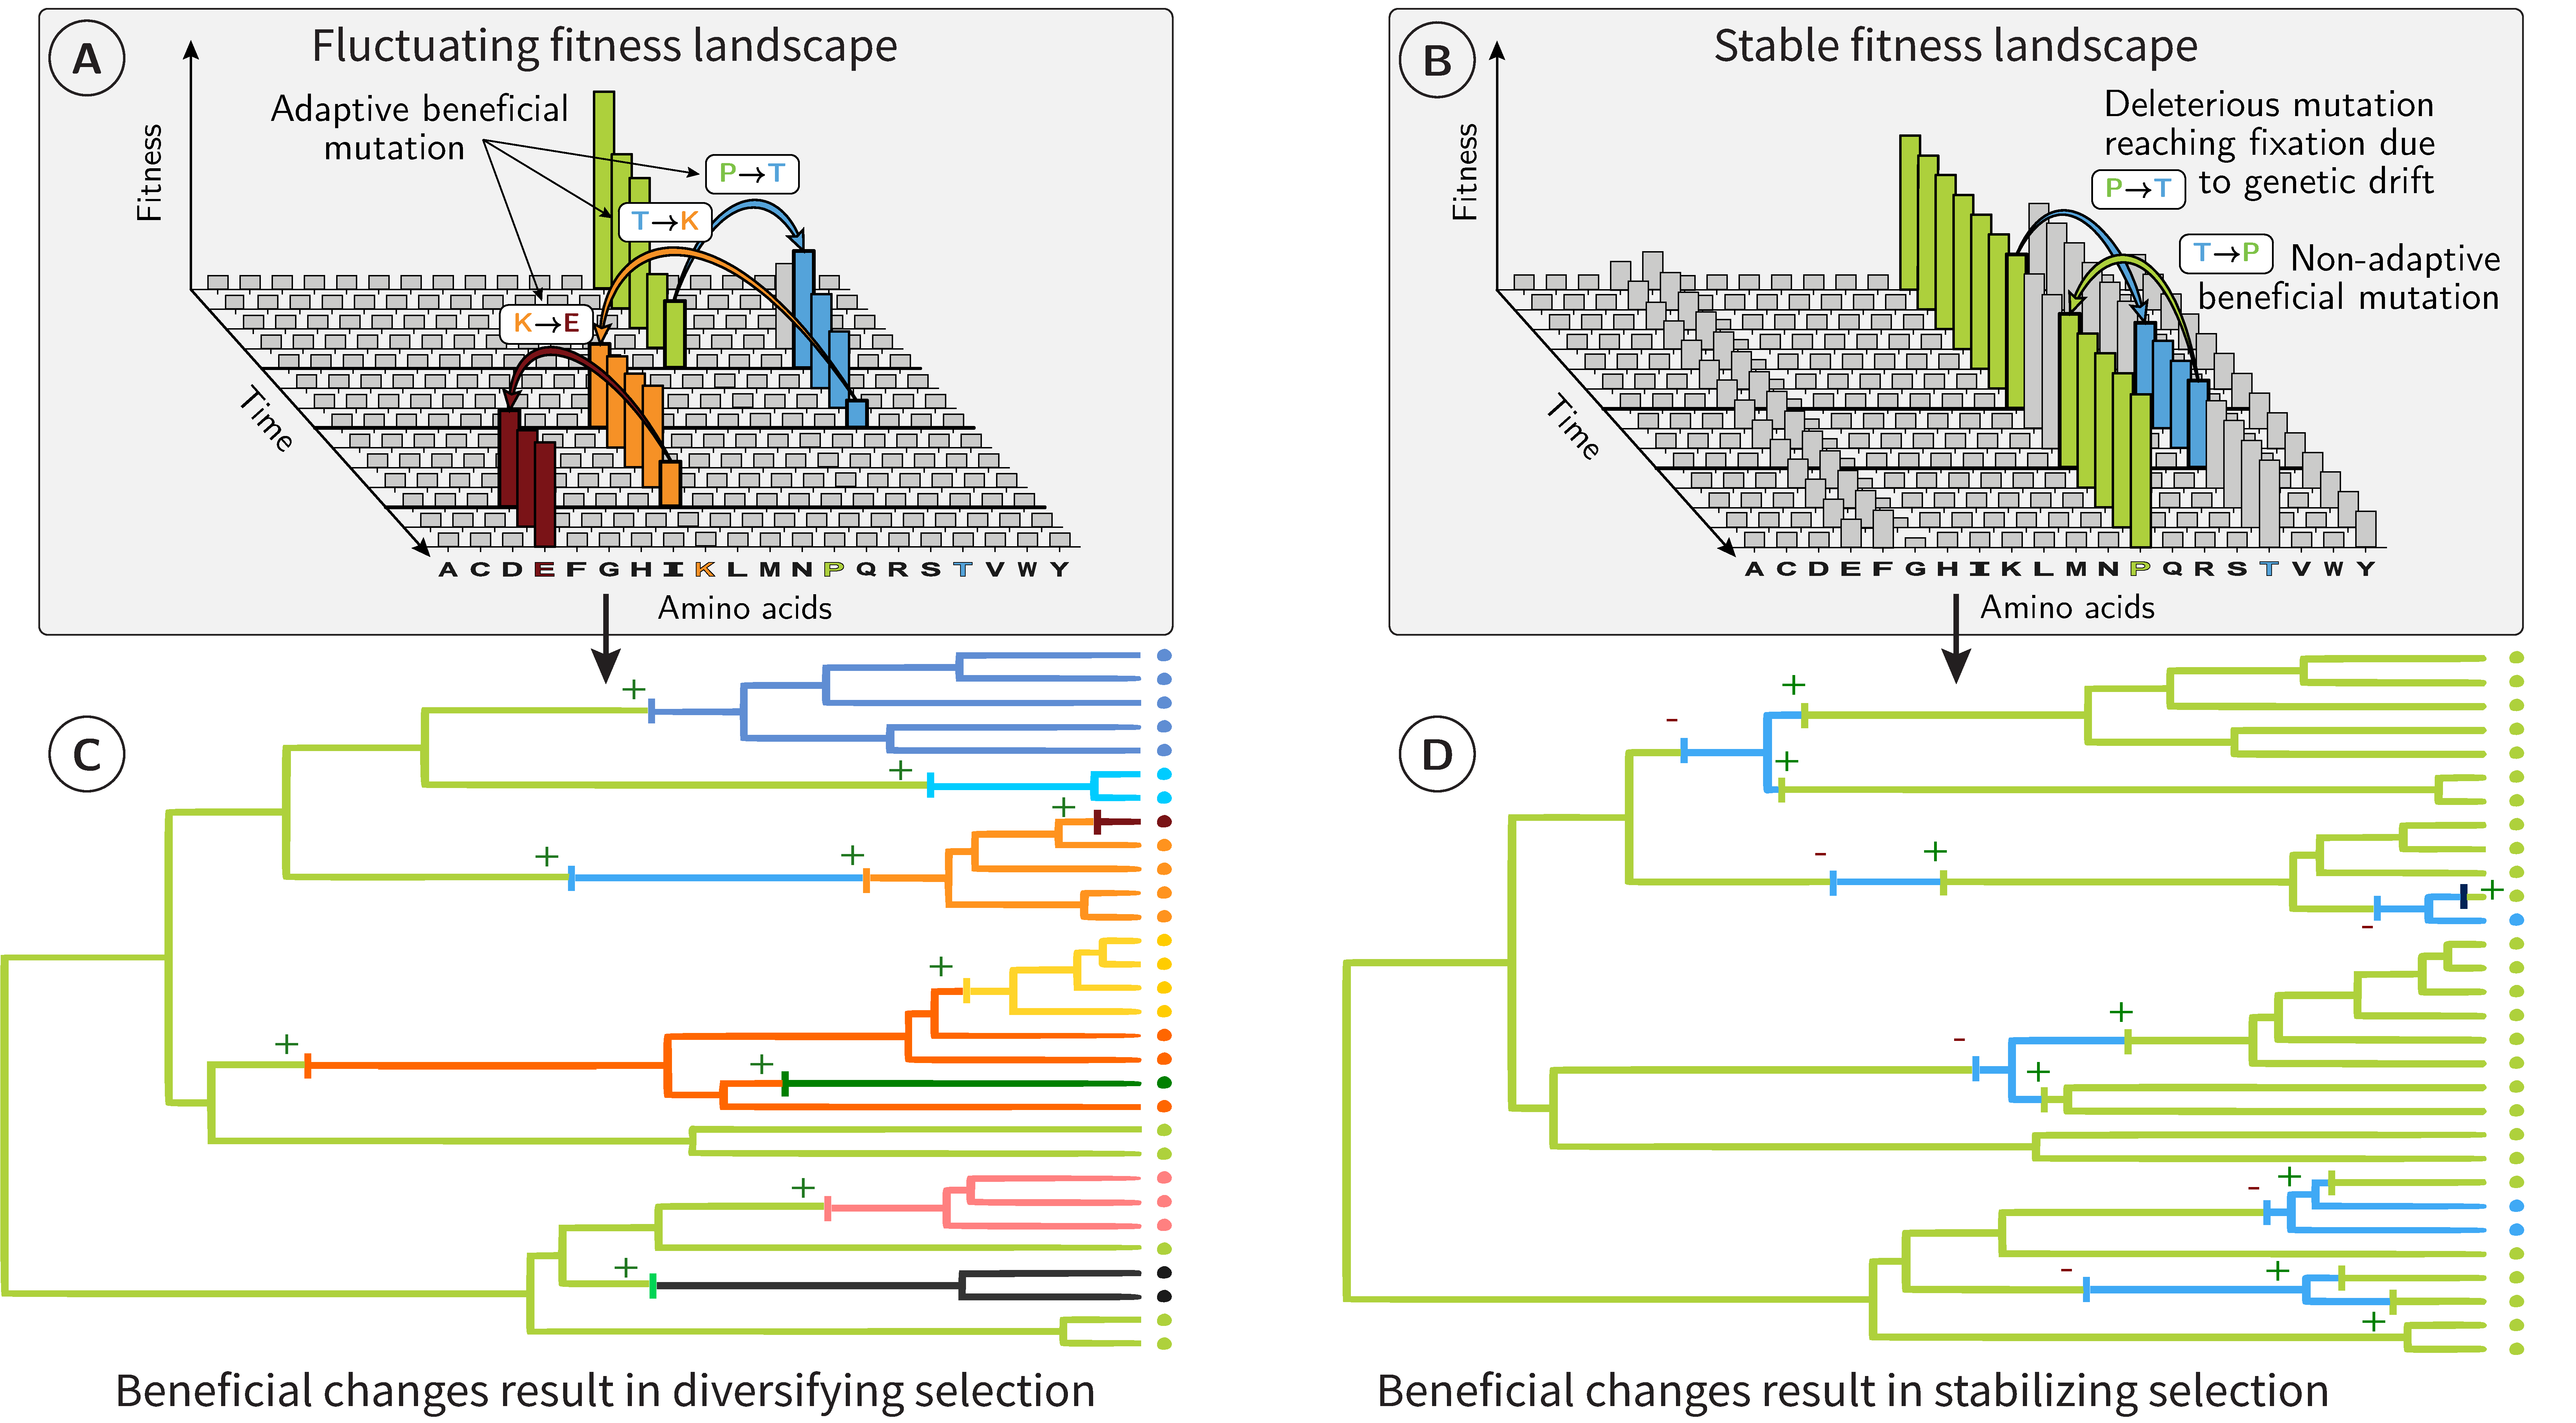
\includegraphics[width=\textwidth, page=1] {artworks/figure.fitness-landscape}
        \caption{
            Panel A and B: at a given site inside a protein-coding DNA sequence, the different amino acids (x-axis) have different fitnesses (y-axis).
            Under a fluctuating fitness landscape (panel A), these fitnesses are changing with time.
            The protein sequence is always lagging behind the moving target defined by the amino acid fitnesses, and since substitutions are accepted preferentially if they are in the direction of this target, substitutions are on average adaptive.
            At the phylogenetic scale (panel C), this phenomena promotes phenotype diversification across species.
            Under a static fitness landscape (panel B), the protein sequence only fluctuates at the mutation-selection balance.
            All the mutations reaching fixation are either slightly deleterious and reaching fixation due to drift or are advantageous and restoring a more optimal amino acid.
            At the phylogenetic scale (panel D), this phenomena promotes promotes phenotype stability and preserves well established biological systems.
        }
        \label{fig:fitness-landscape}
    \end{figure*}

    \begin{figure*}[!ht]
        \centering
        \includegraphics[width=\textwidth, page=1] {artworks/figure.method}
        \caption{
            Integrating divergence and polymorphism.
            At the phylogenetic level (panel A), the amino-acid Wrightian fitness for each site is estimated from protein-coding DNA alignments using mutation-selection codon models.
            At the population-genetic level (panel B), for each observed single nucleotide polymorphism (SNP) segregating in the population, selection coefficient are computed as the difference in amino-acid fitness between the ancestral and derived variants.
        }
        \label{fig:method}
    \end{figure*}

    To answer these questions, we estimated the fitness landscape of amino-acid for long-term evolution using available multiple sequence alignments between mammalian species\cite{ranwez_orthomam_2007, howe_ensembl_2021}.
    We developed a pipeline to integrate data at the phylogenetic and population scale to estimate divergence and polymorphism, respectively, across the entire exome for 28 populations from 6 genera (\textit{Equus},  \textit{Bos}, \textit{Capra}, \textit{Ovis}, \textit{Chlorocebus} and \textit{Homo}; fig.~\ref{fig:method}A\&B).


    \subsection*{SNPs which are predicted to be advantageous are positively selected at the population scale}


    For each non-synonymous SNP observed at the population level, we predicted its scaled selection coefficient ($\Sphy$) from amino-acid fitnesses estimated at the mammalian scale (fig.~\ref{fig:method}B).
    Then we ask whether the variants that are supposedly advantageous are showing signatures of short term positive selection.
    For example, if a variant is found to be fixed in many mammals but not in ancestral humans, and a mutation in humans is toward the mammalian version, is this mutation advantageous for the individual carrying it?
    At the population level (e.g. in humans of Asian descent in fig.~\ref{fig:homo-afr-results}), we divided all observed SNPs in 5 classes of predicted selection coefficient: severely deleterious with $\divStrongDel$, deleterious with $\divDel$, weakly deleterious with $\divWeakDel$, weakly advantageous with $\divWeakAdv$ and advantageous with $\divAdv$ (fig.~\ref{fig:homo-afr-results}B).
    In each of theses classes, SNPs are then grouped by the number of derived alleles in the population (fig.~\ref{fig:homo-afr-results}C), generating a so called site-frequency spectrum (SFS).
    Compared to synonymous mutations which are supposedly neutral (black line in fig.~\ref{fig:homo-afr-results}C), mutations predicted to be deleterious (blue and green lines in fig.~\ref{fig:homo-afr-results}C) are underrepresented at high frequencies in the population, a signature of ongoing purifying selection.
    However, these observations remain qualitative.

    To obtain a quantitative estimate of the distribution of selection coefficient for each category of SNPs, we used the model polyDFE\cite{tataru_inference_2017, tataru_polydfe_2020}.
    This model uses the count of derived alleles for each frequency class of the SFS to infer the distribution of fitness effects (DFE) of the region under study.
    The model uses both the number of sites ($L$) for each category (fig.~\ref{fig:homo-afr-results}A, see Material and Methods), and the counts of synonymous derived allele as a neutral model, which allow to control for demographic effects, and polarization errors when inferring the ancestral state.
    These population-based models cannot give a specific estimate of the selection coefficient at the population-genetic scale ($\Spop$) for each SNP, but by gathering information across many SNPs, these models can estimate the proportion of advantageous mutations ($\PpolyAdv$), of nearly-neutral mutations ($\PpolyNeutral$) and of deleterious mutations ($\PpolyDel$) (fig.~\ref{fig:homo-afr-results}D).
    We found that SNPs predicted to be deleterious given their selection coefficient $\Sphy$ across mammals are effectively purged at the population-genetic scale, demonstrating that purifying selection is largely predictable and amino acids with low fitness across mammals are effectively purged away in each population.
    Notably, SNPs predicted to be advantageous given their selection coefficient $\Sphy$ are indeed under positive selection at the population-genetic scale, confirming that there is a local ongoing selection towards amino acids that are restoring the optimally functioning protein.
    In between these two extremes, mutations predicted to be weakly selected (cyan and orange in fig.~\ref{fig:homo-afr-results}) are effectively composed of neutral, positively and negatively selected mutations.

    We replicated such experiment across 28 populations (fig.~\ref{fig:heatmap}), and found that mutations predicted to be deleterious are indeed purged at the population-genetic scale (blue and green rows in fig.~\ref{fig:heatmap}A).
    However, mutations predicted to be weakly advantageous ($\divWeakAdv$) are composed of a mix of neutral and selected mutations with varying proportions across the different populations (orange row in fig.~\ref{fig:heatmap}B).
    Similarly, mutations predicted to be advantageous are found to be positively selected with varying proportions across populations (red row in fig.~\ref{fig:heatmap}C).
    These variable proportions between populations can be explained by the effective number of individuals in the population ($\Ne$), a major driver of selection efficacy.
    Since $\Ne$ is not directly measurable, a reasonable proxy usually used is the synonymous diversity (see material and methods).
    We thus ordered populations by their levels of synonymous diversity (fig.~\ref{fig:diversity}A) and confirmed that higher synonymous diversity is typically accompanied by a smaller proportion of neutral mutations.
    This result suggests that populations with higher diversity (e.g.~\textit{Bos} or \textit{Ovis}) are more likely to discriminate between advantageous and deleterious mutations (fig~S1-S5).
    Alternatively stated, mutations in populations with low diversity (e.g.~\textit{Homo}) are effectively nearly-neutral and behave as would a neutral mutation.
    %, especially for mutations already predicted to be nearly-neutral at the phylogenetic scale (fig~S8-S9).
    This result is qualitatively in accordance with the nearly-neutral theory of evolution which argues that mutations are less efficiently selected for in small populations.

    Finally, we reconstructed the substitutions in the terminal branches of the phylogenetic tree to determine the distribution of their selection coefficients.
    For each population with available polymorphism data, we first reconstructed the ancestral sequence (which is different than the reference sequence), then we mapped the substitutions from the last genus split to this reconstructed ancestral sequence.
    In these populations, we show that out of all polarized substitutions in the branches, between 10 and 17\% of all substitutions have an $\Sphy > 1$ (table S1) and between 22 and 42\% of all substitutions have an $\Sphy > 0$ (table S2).
    Most importantly, there is clear signal that the substitutions with an $\Sphy > 1$ have been positively selected since their ratio of non-synonymous over synonymous divergence, a ratio called $\dnds$, is between 1.05 and 1.81 in the different populations (table S1), meaning that mutations with $\Sphy > 1$ reach fixation more frequently that synonymous mutations (supposedly neutral).
    %This also means that the ratio $\dnds$ usually used to detect adaptation while relying on substitutions between close species\cite{mcdonald_adaptative_1991, galtier_adaptive_2016} or at the phylogenetic scale\cite{goldman_codonbased_1994, yang_codonsubstitution_2002} is overestimated.
    These observed substitutions are likely to have been positively selected because they restored a more optimal state, not because they are driving innovations to a new environment or a new function.

    \subsection*{A large proportion of advantageous mutations are non-adaptive}

    We then tried to estimate the proportion of restoring mutations among advantageous ones.
    Since adaptation does not fit the fitness predictions, the proportion of adaptive mutation is expected to be the same among SNPs which are predicted to be advantageous, and among SNPs which are predicted to be deleterious.
    Thus the proportion of advantageous mutations among SNPs which are predicted to be deleterious directly correspond to the proportion of all mutations which are adaptive.
    So if we divide the proportion of mutations which are predicted to be advantageous among supposedly deleterious SNPs by the proportion of mutations which are predicted to be advantageous among all SNPs, we directly get the proportion of mutations which are adaptive among advantageous ones.
    It results that 20 to 40\% of advantageous mutations are due to maintenance positive selection (fig~\ref{fig:diversity}B \& table S2).

    In a similar way, we can consider that the total $\dnds$ encompasses the rate of evolution of deleterious, restoring and adaptive substitutions.
    Then, the $\dnds$ computed exclusively on non-synonymous sites with a $\Sphy < 0$ only represent the rate of evolution of solely deleterious and adaptive substitutions, discarding the restoring substitutions by construction.
    Thus, if we divide the $\dnds$ estimated on all substitutions, by the one estimated only on substitutions predicted to be deleterious, we directly get the proportion of the rate of evolution which is due to maintenance positive selection.
    This way, we estimated that between 20 and 25\% of the evolutionary rate is due to maintenance positive selection (fig~\ref{fig:diversity}C \& table S2).

    Interestingly, the proportion of restoring mutations among advantageous ones and the proportion of the rate of evolution explained by maintenance positive selection do not show a clear relationship with the synonymous diversity (a proxy for the effective population size) (fig.~\ref{fig:diversity}B and C).
    Indeed, the relationship between $\Ne$ and the proportion of restoring mutations is not trivial and should highly depend on time scales.
    A population which experienced a high long term $\Ne$ in the past is supposed to be closer to the optimal state (under a stable fitness landscape), and should not leave much space for restoring mutations.
    On the other hand a high short term $\Ne$ will induce more extreme fitness effects and a larger proportion of otherwise effectively neutral restoring mutations will be positively selected, thus increasing the proportion of restoring mutations.
    Overall, the proportion of restoring mutations is expected to be more dependent on effective population size contraction or expansion rather than on the short term effective population size captured by the synonymous diversity.

    \begin{figure*}[!ht]
        \centering
        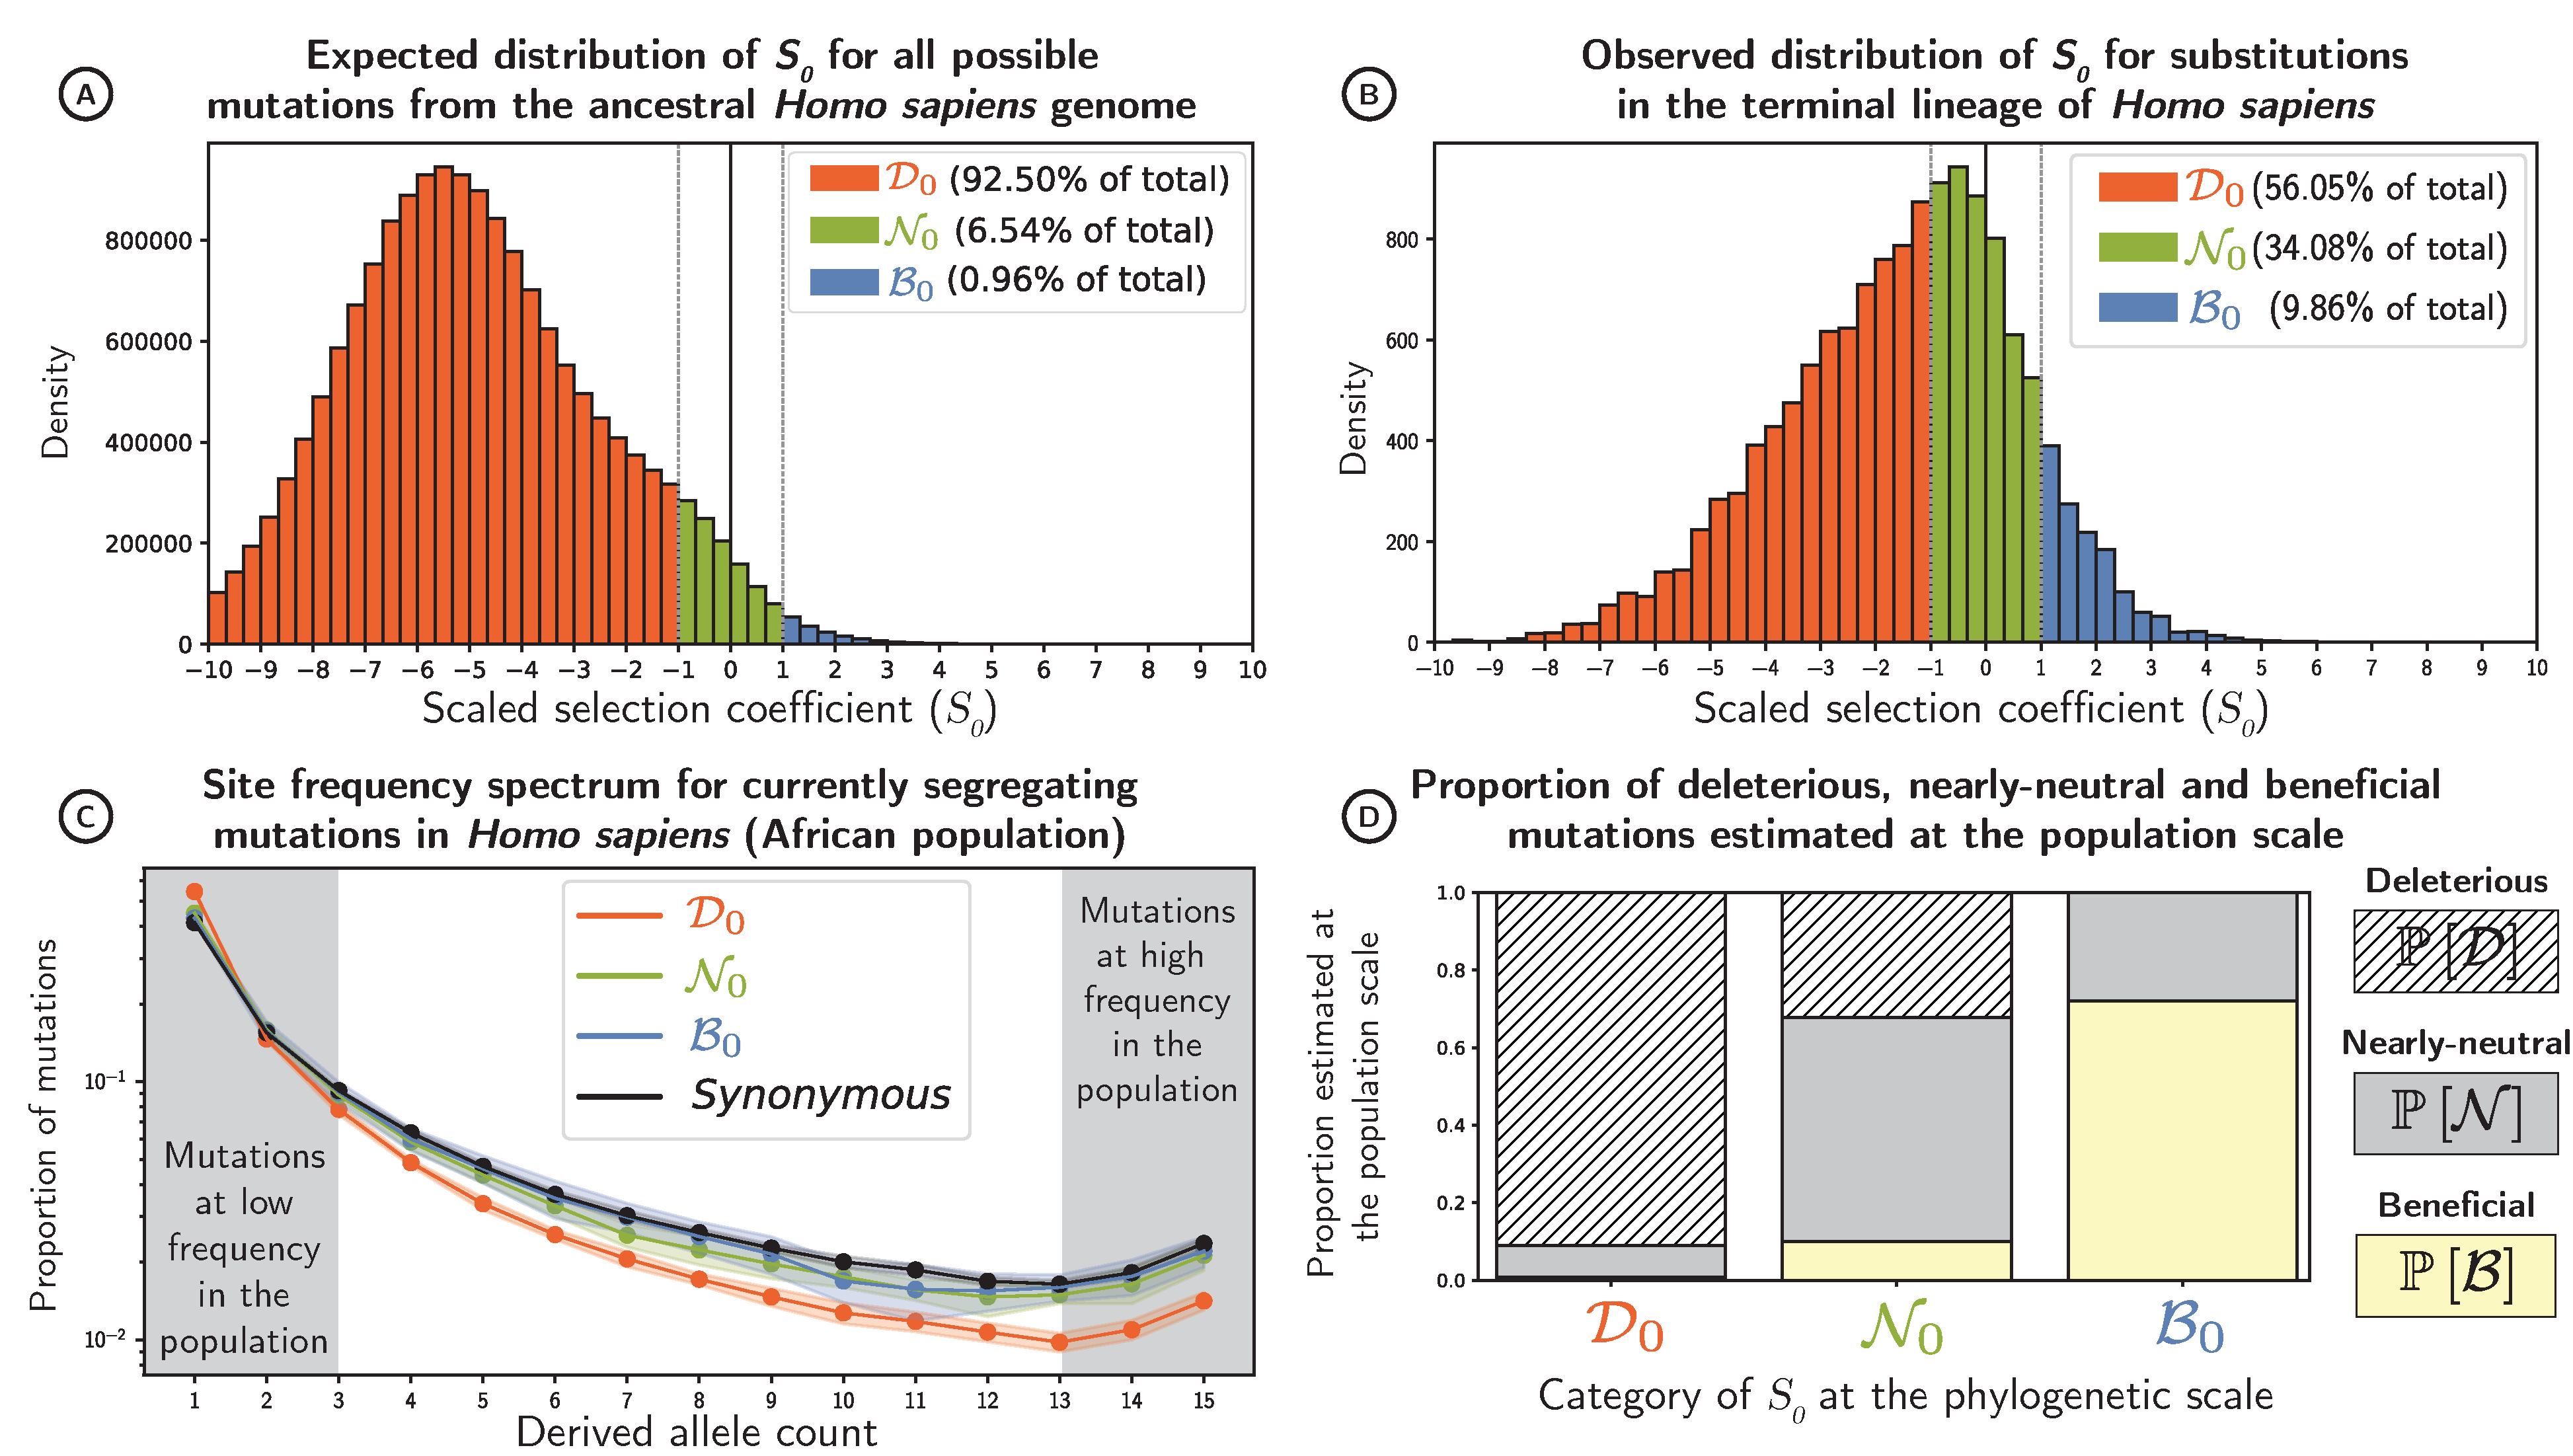
\includegraphics[width=\textwidth, page=1] {artworks/figure.homo-afr-results}
        \caption{
            Panel A: Histogram of predicted selection coefficients ($\Sphy$) for all possible mutations away from the ancestral human genome, giving the number of sites ($L$, in y-axis) across the genome with a given $\Sphy$.
            Mutations are divided into 5 classes: severely deleterious (blue), deleterious (green), weakly deleterious (light green), weakly advantageous (yellow) and advantageous (red).
            Panel B. Histogram of predicted selection coefficients ($\Sphy$) for all observed mutations in a sample of 8 individuals (out of 512 in the original dataset) of African descent.
            If they are less mutations observed than expected, this class is thus undergoing purifying selection.
            Panel B: The site-frequency spectrum (SFS) represents the proportion of mutations (y-axis) with a given number of derived alleles in the population (x-axis).
            SFS are drawn for a random sample of 16 alleles (mean in solid line and standard deviation in filled color) for each class of selection coefficient and for synonymous mutations which are supposedly neutral (black).
            At high frequencies, supposedly severally deleterious mutations are underrepresented.
            Panel D. For each class of selection (and for the set of all non-synonymous mutations), information from the SFS and the expected total mutation rate are combined at the population-genetic scale to estimate the proportion of advantageous mutations $\PpolyAdv$, of nearly-neutral mutations $\PpolyNeutral$ and of deleterious mutations $\PpolyDel$.
        }
        \label{fig:homo-afr-results}
    \end{figure*}

    \begin{figure*}[!ht]
        \centering
        \includegraphics[width=\textwidth, page=1] {artworks/figure.heatmap}
        \caption{
            Reproducibility of results shown in figure~\ref{fig:homo-afr-results} in 28 populations across 6 genera.
            For each class of selection at the phylogenetic scale ($\Sphyclass \in \{ \divStrongDel, \divDel,  \divWeakDel,  \divWeakAdv, \divAdv \}$, in rows), site-frequency spectra and total number of sites are combined at the population-genetic scale to estimate the proportion of advantageous mutations ($\PpolyAdv$) in the top panel, of nearly-neutral mutations ($\PpolyNeutral$) in the middle panel and of deleterious mutations ($\PpolyDel$) in the bottom panel.
        }.
        \label{fig:heatmap}
    \end{figure*}

    \begin{figure*}[!ht]
        \centering
        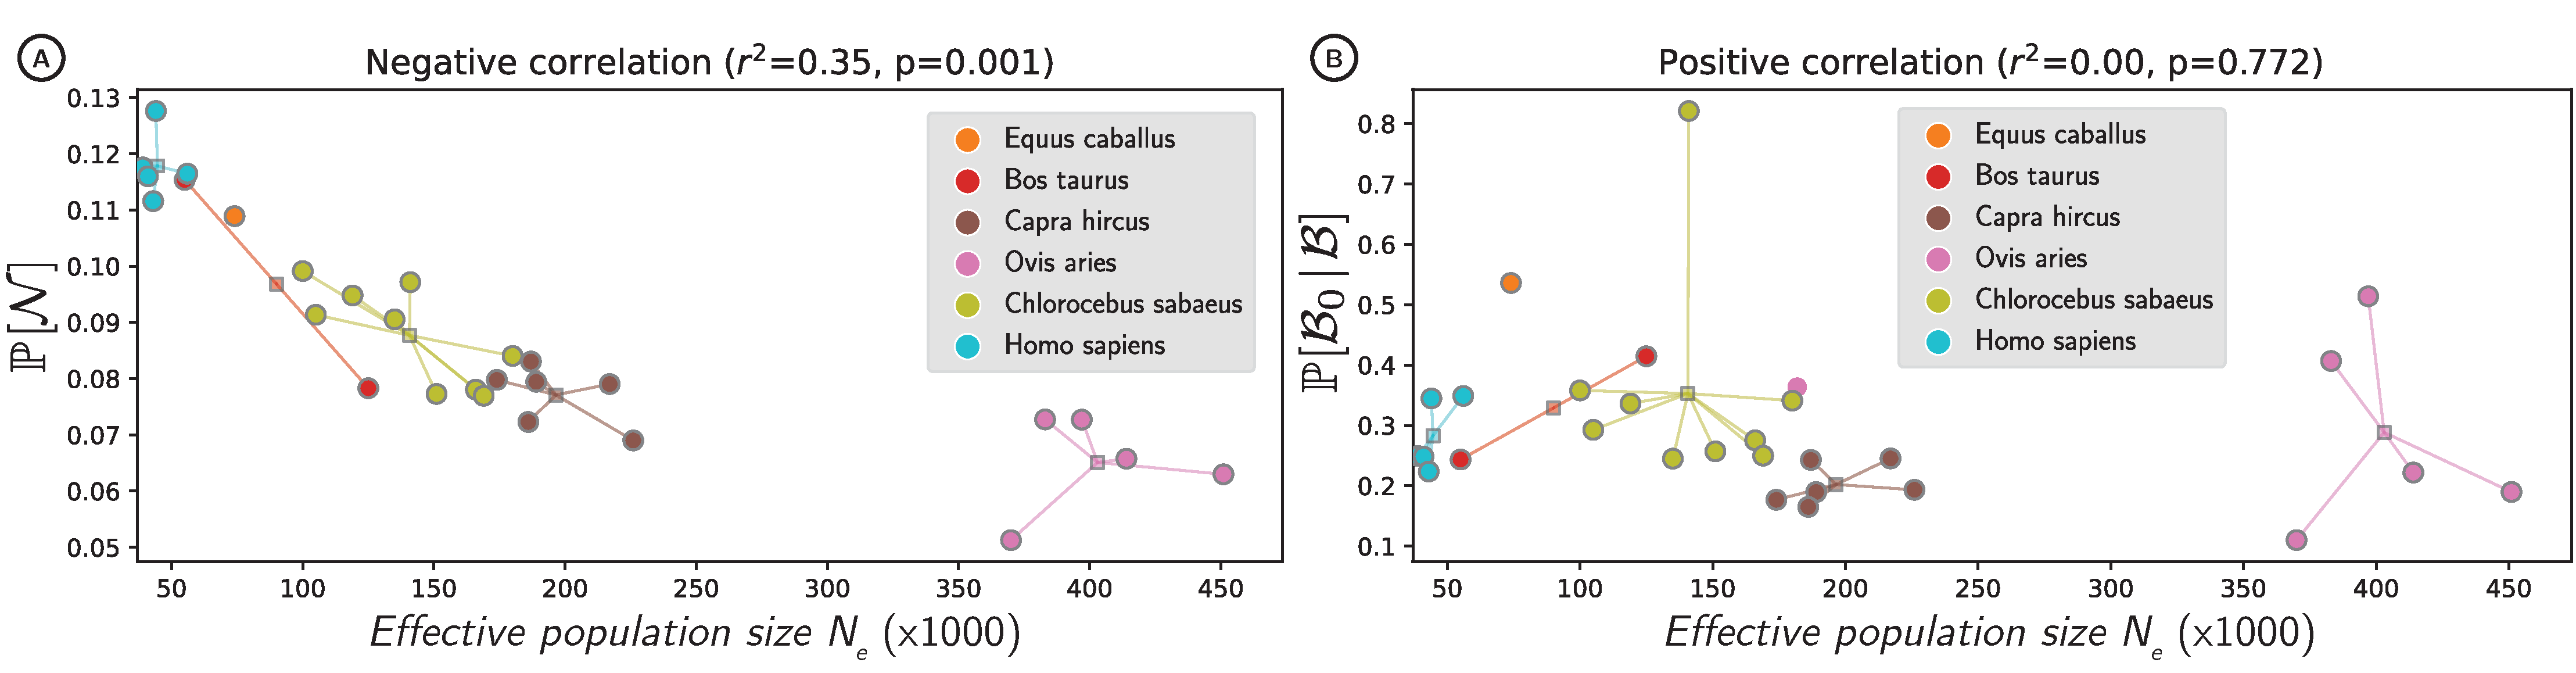
\includegraphics[width=\textwidth, page=1] {artworks/figure.diversity}
        \caption{
            Panel A. For each population, the proportion of advantageous ($p_+=\PpolyAdv$), nearly-neutral ($\PpolyNeutral$) and of deleterious ($\PpolyDel$) mutations estimated at the population-genetic scale using all SNPs available.
            Population are sorted for increased synonymous diversity.
            Panel B. $R(p_+)=\dfrac{p_+ - p_+(\Sphy < 0)}{p_+}$ is the fraction of non-adaptive advantageous mutations, $p_+$ is compared to its estimation when we had removed all the restoring mutations $p_+(\Sphy < 0)$.
            $R(p_+)$ (y-axis) is shown as a function of the synonymous diversity (Watterson $\theta_w$ in x-axis).
            Panel C. $R(\dnds)=\dfrac{\dnds - \dn(\Sphy < 0) / \ds}{\dnds}$ is the fraction of divergence ($\dnds$) that is due to maintenance positive selection, where $\dnds$ is compared to the estimated divergence when we removed the restoring substitutions $\dn(\Sphy < 0)/\ds$.
            $R(\dn)$ (y-axis) is shown as a function of the synonymous diversity (Watterson $\theta_w$ in x-axis).
        }
        \label{fig:diversity}
    \end{figure*}

    % Our study is a bridge between phylogenetic and population genetics
    From a theoretical evolution perspective, we have found that we can use phylogenetic signals and mutation-selection codon models to predict the selection coefficient of a mutation.
    However, we so far assumed no changes in effective population size while it has been established that population size changes have a major effect on selection dynamics\cite{lanfear_population_2014, jones_shifting_2017, platt_protein_2018}.
    Estimating effective population sizes along with fitness landscapes is possible\cite{latrille_inferring_2021}, but is, for the moment, too computational intensive to be performed genome-wide\cite{latrille_inferring_2021}.
    Hybrid mutation-selection and $\omega$-based codon models could provide a way forward\cite{brevet_reconstructing_2021}.
    Moreover, SIFT scores based on amino-acid alignments across species have also been found to be informative of the selection pressure exerted at the population scale\cite{chen_hunting_2021}.
    Accordingly, our study shows that sites with a higher SIFT score at the phylogenetic scale are more positively selected in the different populations (supp.\ mat\  section SIFT scores).
    In practice, SIFT scores are more coarse grained, with for example a bulk of mutations with a score of 1.0 (the highest), and does not provide a boundary between advantageous and deleterious mutations, nor are they based on a population-genetics formalism.

    Biologically, another mechanism which generate maintenance positive selection is compensatory mutations, which are repairing damage caused by deleterious mutations at another site in the genome and generating a widespread signal of non-adaptive positive selection\cite{hartl_compensatory_1996, pollock_strong_2014, starr_epistasis_2016}.
    In our study we focused on mutations restoring the more optimal ancestral state at a given site, not accounting for compensatory mutations since we assumed a model of fitness landscape without epistasis, providing a reasonable estimate of average fitness profiles\cite{youssef_consequences_2020}.
    But most importantly, we argue that our estimation of the amount of maintenance positive selection is an underestimation, and that accounting for compensatory mutations by means of epistasis would mechanically increase that amount.
    Indeed, a fluctuating fitness landscape due to an external forces (e.i. changes in environment) results in an acceleration of the rate of evolution\cite{ rodrigue_detecting_2017, rodrigue_bayesian_2021} which generates epistatic mutations that are immediately beneficial\cite{gong_epistatically_2014}.
    On the contrary, pervasive epistasis generates the opposite, an entrenchment\cite{goldstein_evolutionary_2004, goldstein_nonadaptive_2015} resulting in a slowing down of the rate evolution\cite{rodrigue_detecting_2017, patel_epistasis_2022} or a standstill\cite{youssef_evolution_2022}.
    In other words, under pervasive epistasis, finding empirical evidence for restoring mutations is harder since restoring mutations become less and less likely to occur over time\cite{goldstein_nonadaptive_2015, goldstein_sequence_2017, park_epistatic_2022}.
    Our study thus shows that restoring mutations should not be overlooked, and we argue that both restoring and compensatory mutations play an important role in preventing our genome from collapsing under a mutation load.

    %Second, epistasis is not modelled while it can have drastic consequences on the change in fitness landscape\cite{latrille_quantifying_2021}.
    %Some models using Direct Coupling Analysis (DCA) can infer coevolution between sites, and thus provide a fitness score for amino acids which depends on other sites of the sequence\cite{bisardi_modeling_2022}.
    %However, as SIFT scores, the scores given by DCA are not formalized in terms of selection coefficients and thus are hard to interpret in terms of population genetics, while also neglecting the underlying phylogeny and mutational biases.
    %Relaxing both assumptions are computationally intensive\cite{rodrigue_site_2005, kleinman_statistical_2010}, and would require new mutation-selection models and optimization techniques to be able to manipulate genome-wide datasets..

    % Alternatively at the DNA level, $\omega$-based codon model use the ratio of non-synonymous over synonymous substitution as signature of selection\cite{goldman_codonbased_1994, yang_codonsubstitution_2002}, taking into account the mutational bias and the underlying phylogeny.
    % We also show that sites with higher $\omega$ are more positively selected in the different populations (supp.\ mat\  section 3).
    % However, even sites which are supposedly under pervasive positive selection at the phylogenetic scale ($\omega>1$) are not necessarily positively selected in the populations.
    %Most importantly, such models do not leverage the information of the source and target amino acid involve in the mutation, and thus cannot be used to estimate the non-adaptive part of positive selection.
    %Altogether, we here show that mutation-selection codon models formalize a bridge between phylogenetics and population genetics models, but both ends have its limitation and could be improved.

    At the population-genetic level, our study relied on models with some shortcomings, such that there is no consensus on the expected shape of the DFE\cite{welch_divergence_2008, bataillon_effects_2014}, although it has been found to be reliably constant between species\cite{castellano_comparison_2019}.
    The model we used allows the inference of a full DFE, modelling the negative part of the DFE as a gamma distribution, and the positive part as an exponential distribution.
    However, when we aggregate SNPs that are expected to be strongly deleterious or strongly advantageous, the model struggles to fit their DFE to a gamma or an exponential distribution.\cite{brevet_reconstructing_2021}
    As a result, while the proportions of negative/weak/positive mutations stays reliable, the mean values for selection coefficients ($\Spop$) estimated by polyDFE become biologically absurd ($\Spop \ll -10^3$).
    Such effect is not found for neutral SNPs and a method to accurately estimate the mean value of selection coefficients from SFS without assuming any shape for the DFE remains yet to be developed.
    Aside from methodological limitations, the mammalian case study might also not be representative of other clades.
    Indeed, mammals have relatively small long term population sizes, which allow large amounts of deleterious mutations to be fixed, and thus, there are a lot of opportunities for maintenance positive selection to arise.
    It would thus be of great interest to reproduce our experiment with other clades, such as \textit{Drosophila} or birds which tend to have higher effective population size.
    It would also be interesting to have access to more shallow but wider phylogenies to increase the resolution of our predictions.

    From a structural biology perspective, we have found that proteins are not optimal for their fitness, which has been proved for their kinetics and thermodynamics\cite{taverna_why_2002, goldstein_evolution_2011}.
    We argue that mutation-selection models are thus a mandatory tool in evolutionary biology to detect and quantify adaptation since they genuinely take into account the tug-of-war between scarce advantageous mutations likely to reach fixation and a bulk of deleterious mutations eventually reaching fixation due to their sheer mass.
    Indeed, these models can be used as a null model to predict the expected rate of evolution of proteins\cite{spielman_relationship_2015, dosreis_how_2015} under a stable fitness landscape.
    A departure from this model indicates that proteins are evolving under a changing fitness landscape\cite{rodrigue_detecting_2017, tamuri_mutationselection_2021} and is a signal of pervasive adaptive evolution\cite{rodrigue_bayesian_2021} or of pervasive epistasis\cite{rodrigue_detecting_2017}.


    \section*{Acknowledgments}
    \label{sec:acknowledgment}
    We gratefully acknowledge the help of Diego A. Hartasánchez Frenk for his advice and review concerning this manuscript.
    This work was performed using the computing facilities of the CC LBBE/PRABI\@.
    This study makes use of data generated by the NextGen Consortium.
    The European Union’s Seventh Framework Programme (FP7/2010-2014) provided funding for the project under grant agreement no 244356 - “NextGen”.
    \textbf{Funding:}
    Université de Lausanne; Agence Nationale de la Recherche, Grant ANR-19-CE12-0019 / HotRec.
    \textbf{Author contributions:}
    Original idea: T.L.\ and J.J.;
    Model conception: T.L., J.J.\ and N.S.;
    Code: T.L.;
    Data analyses: T.L.\ and J.J.;
    Interpretation: T.L., J.J.\ and N.S.;
    First draft, editing and revisions: T.L., J.J.\ and N.S.;
    Project management and funding: N.S\@.
    \textbf{Competing interests:}
    The authors declare no conflicts of interest.
    \textbf{Data and materials availability:}
    Snakemake pipeline, analysis scripts and documentation are available at \href{https://github.com/ThibaultLatrille/SelCoeff}{github.com/ThibaultLatrille/SelCoeff}.


    \section{Material \& Methods}
    \label{sec:methods}

    \subsection{Phylogenetic dataset}

    Protein-coding DNA sequences alignments in placental mammals and their corresponding gene trees were extracted from the \href{https://www.orthomam.univ-montp2.fr}{OrthoMaM} database. It contained a total of $116$ mammalian reference sequences in v10c\cite{ranwez_orthomam_2007, douzery_orthomam_2014, scornavacca_orthomam_2019}.
    Genes located on the X, Y chromosomes and the mitochondrial genome were discarded from the analysis, because the level of polymorphism, which is necessary in the population-based analyses, is expected to be different in these three genomic regions.
    Sequences of species for which we used poppulation-level polymorphism (see below), as well as their sister species, were removed from the analysis to ensure independence between the data used in the phylogenetic and population genetic scale.
    Altogether, we analyzed $14,509$ protein-coding DNA sequences for at most $87$ sequences of placental mammals.

    \subsection{Selection coefficient ($\Sphy$) in phylogeny-based method}
    \label{subsec:s-phylogeny-method}

    We analyzed the phylogenetic level data using mutation-selection models. These models assume that the protein-coding sequence are at mutation-selection balance under a fixed fitness landscape characterized by a fitness vector over the $20$ amino-acid at each site\cite{yang_mutationselection_2008, halpern_evolutionary_1998, rodrigue_mechanistic_2010}.
    Mathematically, the rate of non-synonymous substitution from codon $a$ to codon $b$ ($q_{a \mapsto b}^{(i)}$) at site $i$ of the sequence is equal to the rate of mutation of the underlying nucleotide change ($\mu_{a \mapsto b}$) multiplied by the scaled probability of fixation of the mutation ($\proba_{a \mapsto b}^{(i)}$).
    The probability of fixation depends on the difference of scaled fitness of the amino-acid encoded by the mutated codon ($F_b^{(i)}$) and the amino-acid encoded by the original codon ($F_a^{(i)}$) at site $i$\cite{wright_evolution_1931, fisher_genetical_1930}.
    The rate of substitution from codon $a$ to $b$ at a site $i$ is thus:
    \begin{equation}
        \begin{dcases}
            q_{a \mapsto b}^{(i)} & = 0 \text{ if codons $a$ and $b$ are more than one mutation away,} \\
            q_{a \mapsto b}^{(i)} & = \mu_{a \mapsto b} \text{ if codons $a$ and $b$ are synonymous,} \\
            q_{a \mapsto b}^{(i)} & = \mu_{a \mapsto b} \dfrac{F_b^{(i)} - F_a^{(i)}}{1 - \e^{F_a^{(i)} - F_b^{(i)}}} \text{ if codons $a$ and $b$ are non-synonymous}.
        \end{dcases}
    \end{equation}
    Fitting the mutation-selection model on a sequence alignment leads to an estimation of the mutation rate matrix ($\UniDimArray{\mu}$) as well as the 20 amino-acid fitness landscape ($\UniDimArray{F^{(i)}}$) at each site $i$.
    The selection coefficient for a mutation from codon $a$ to codon $b$ at site $i$ is defined :
    \begin{equation}
        S_{a \mapsto b}^{(i)} = \Delta F^{(i)} = F^{(i)}_{b} - F^{(i)}_{a}.
    \end{equation}
    In the manuscript and the following material, the source ($a$) and target ($b$) codons as well as the site ($i$) are implicit and thus never explicitly written.
    We ran the Bayesian software \href{https://github.com/bayesiancook/bayescode}{BayesCode} on each protein-coding DNA alignment\cite{lartillot_phylobayes_2013, rodrigue_detecting_2017, rodrigue_bayesian_2021}.
    We ran a Markov chain Monte-Carlo (MCMC) analysis during $2000$ generations, with a burn-in period of $1000$ generations, to obtain posterior mean estimates of the amino-acid fitness landscape ($\UniDimArray{F^{(i)}}$) at each site $i$\@.

    \subsection{Polymorphism dataset}
    \label{subsec:polymorphism-dataset}

    We retrieved the genetic variants representing the population level polymorphism from the following species and respective available datasets: \textit{Equus caballus} (EquCab2 assembly in the EVA study PRJEB9799\cite{alabri_whole_2020}), \textit{Bos taurus} (UMD3.1 assembly in the NextGen project: \url{https://projects.ensembl.org/nextgen/}), \textit{Ovis aries} (Oar\_v3.1 assembly in the NextGen project: \url{https://projects.ensembl.org/nextgen/}), \textit{Capra Hircus} (CHIR1 assembly in the NextGen project: \url{https://projects.ensembl.org/nextgen/}, liftover to the ARS1 assembly), \textit{Chlorocebus sabaeus} (ChlSab1.1 assembly in the EVA project PRJEB22989\cite{svardal_ancient_2017}), \textit{Homo sapiens} (GRCh38 assembly from the 1000-genome project\cite{consortium_integrated_2012, the1000genomesprojectconsortium_global_2015}).
    In total, we analyzed 28 populations across the 6 different species with polymorphism data.
    Genetic variants that were not found within a gene were not used in further analyses.
    We also did not analyzed insertions and deletions and focused only on Single Nucleotide Polymorphisms (SNPs) with a single mutant allele.
    Finally, stop codon mutants were also discarded.

    Each SNP (chromosome, position, strand) in the focal species was matched to its relative position (chromosome, position, strand) in the protein-coding DNA alignment by first converting the genomic positions to relative position in the coding sequence (CDS) using gene annotation files (GTF format) downloaded from Ensembl (\url{ensembl.org}).
    We then verified that the SNP downloaded from Ensembl were matching the reference in the CDS (FASTA format).
    Second, the relative position in the CDS was converted to position in the multiple sequence alignment (containing gaps) from OrthoMaM database\cite{ranwez_orthomam_2007, douzery_orthomam_2014, scornavacca_orthomam_2019} by doing a global pairwise alignment, using the Biopython function pairwise2, between the CDS fasta and the sequence found in the alignment.
    This conversion from genomic position to position in the alignment is only possible if the assembly used for SNP calling is the same as the one used in the alignment, the GTF annotations and the FASTA sequences.

    SNPs were polarized using the $3$ closest outgroups found in the OrthoMam alignment with est-usfs v2.04\cite{keightley_inferring_2018}.
    For populations containing more than $8$ individuals, the site-frequency spectrum (SFS) was subsampled down to $16$ chromosomes ($8$ diploid individuals) without replacement (hyper-geometric distribution) to alleviate the effect of different sampling depth in the 28 populations.

    We developped a Snakemake pipeline to integrate polymorphism and divergence data with custom scripts written in python 3.9.

    \subsection{Selection coefficient ($\Spop$) in population-based method}
    \label{subsec:s-polymorphism-method}
    The probability to sample an allele at a given frequency (before fixation or extinction) is informative of its scaled selection coefficient at the population scale ($\Spop$).
    Pooled across many sites, the SFS provides therefore information on the underlying $\Spop$ of mutations.
    However, estimating a single $\Spop$ for all sampled mutations is biologically unrealistic and a distribution of fitness effects of mutations (DFE) is usually assumed~\cite{eyre-walker_distribution_2006, eyre-walker_estimating_2009}.
    In this study, we used the software polyDFE\cite{tataru_inference_2017, tataru_polydfe_2020}, which used a mixture of a $\Gamma$ and Exponential distributions to model the DFE of non-synonymous mutations, while synonymous mutations are considered neutral.
    The model estimates the parameters $\Spop_d$ , $b$, $p_b$ and $\Spop_b$ for non-synonymous mutations as:
    \begin{equation}
        \phi \left( \Spop; \Spop_d , b, p_b, \Spop_b \right) =
        \begin{dcases}
            \left( 1 - p_b \right) f_{\Gamma}(-\Spop; -\Spop_d, b) & \text{ if $\Spop \leq 0$,} \\
            p_b f_{e}(\Spop; \Spop_b) & \text{ if $\Spop > 0$,} \\
        \end{dcases}
    \end{equation}
    where $\Spop_d \leq -1 $ is the estimated mean of the DFE for $\Spop \leq 0$,
    $b \geq 0.4$ is the estimated shape of the $\Gamma$ distribution,
    $0 \leq p_b \leq 1$ is the estimated probability that $\Spop > 0$,
    $\Spop_b \geq 1$ is the estimated mean of the DFE for $\Spop > 0$,
    and $f_{\Gamma}(x; m, b)$ is the density of the $\Gamma$ distribution with mean m and shape b, while $f_{e}(x; m)$ is the density of the Exponential distribution with mean $m$.
    Once the DFE was fitted to the data, the proportion of advantageous ($\PpolyAdv$), nearly-neutral ($\PpolyNeutral$) and deleterious mutations ($\PpolyDel$) were given as:
    \begin{align}
        p_+ = \PpolyAdv &= p_b \int_{1}^{+\infty} f_{e}(\Spop; \Spop_b) \der \Spop,  \\
        \PpolyNeutral &= p_b \int_{0}^{1} f_{e}(\Spop; \Spop_b) \der \Spop + \left( 1 - p_b \right) \int_{0}^{1} f_{\Gamma}(\Spop; -\Spop_d, b) \der \Spop, \\
        \PpolyDel &= \left( 1 - p_b \right) \int_{1}^{+\infty} f_{\Gamma}(\Spop; -\Spop_d, b) \der \Spop.
    \end{align}

    PolyDFE required one SFS for non-synonymous mutations and one for synonymous mutations (neutral expectation), as well as the total mutation rate (i.e.~mutation rate per site multiplied by the number of sites) on which each SFS has been sampled.
    We performed the following four-step procedure to obtain the number of sites for each SFS.
    First, for each population with polymorphism data available, the polarized SNPs (ancestral and derived alleles) were used to reconstruct the ancestral DNA sequence, containing only substitutions and no segregating polymorphisms.
    If a SNP is still segregating in the population, the ancestral version of the SNP is used.
    However, if the derived allele is shared by all individuals in the population, the allele is considered fixed and the derived allele of the SNP is used instead.
    Second, from this reconstructed ancestral sequence, all possible mutations were computed, weighted by the mutation rate between nucleotide ($\mu$), which was estimated at the phylogenetic scale.
    Third, the total mutation rate for synonymous mutations, called $\mu_{\textrm{syn}}$, was estimated as the sum across the whole genome.
    Similarly, the total mutation rate for each class of selection, called  $\mu\left( \Sphyclass \right)$, was estimated as the sum across all non-synonymous mutations if their selection coefficient at the phylogenetic scale ($\Sphy$) was in the class $\Sphyclass$ (e.g. $\Sphyclass = \divAdv$).
    Fourth, the number of sites ($L$) for each class of selection coefficient ($\Sphyclass$) was finally computed as the total number of sites across the genome ($L_{tot}$) weighted by the ratio of the aggregated mutations rates falling in the class ($\mu\left( \Sphyclass \right)$) over the total mutation rate for all possible mutations:
    \begin{align}
        L_{\textrm{non-syn}} \left( \Sphyclass \right) &= L_{tot} \frac{\mu\left( \Sphyclass \right)}{\mu_{tot}}, \\
        L_{\textrm{syn}} &= L_{tot} \frac{\mu_{\textrm{syn}}}{\mu_{tot}}.
    \end{align}
    From the SFS and the number of sites $L$ for both the synonymous and non-synonymous classes, polyDFE estimated the parameters of the DFE $\phi \left( \Spop; \Spop_d , b, p_b, \Spop_b \right)$ using maximum likelihood.

    The fraction of non-adaptive advantageous mutations $R(p_+)$ was computed as the ratio between the difference in the numbers of advantageous mutations ($p_+$), which were due to maintenance positive selection, and the estimated divergence when we removed the restoring substitutions $p_+(\Sphy < 0)$, over $p_+$.
    \begin{equation}
        R(p_+)=\dfrac{p_+ - p_+(\Sphy < 0)}{p_+}
    \end{equation}

    \subsection*{Substitution mapping in the terminal branch}
    \label{subsec:substitution-mapping-in-the-terminal-branch}
    For each gene and for each population with polymorphism data available, the ancestral DNA sequence was reconstructed from ancestral and fixed polymorphism (see previous section).
    Then, using this ancestral DNA reference and the $3$ closest outgroups found in the OrthoMam alignment, we reconstructed the ancestral protein-coding DNA sequences for each node of the 4-leaves tree with the yang M5 codon model (gamma site rate variation) in FastML.v3.11\cite{ashkenazy_fastml_2012}.
    All polarized codon substitutions are then obtained by comparing the ancestral protein-coding DNA sequences before the split to the sister species (closest outgroup) to the ancestral DNA reference for the population of interest (without segregating polymorphism).
    We considered \textit{Ceratotherium simum simum} as \textit{Equus caballus} sister species; \textit{Bison bison bison} as \textit{Bos taurus} sister species; \textit{Pantholops hodgsonii} as \textit{Ovis aries} sister species; \textit{Pantholops hodgsonii} as \textit{Capra Hircus} sister species; \textit{Macaca mulatta} as \textit{Chlorocebus sabaeus} sister species and finally we considered \textit{Pan troglodytes} as \textit{Homo sapiens} sister species.
    The selection coefficient ($\Sphy$) of each substitution is then obtained by comparing the difference in amino-acid fitnesses for each polarized non-synonymous codon substitution, by referring to the site-specific fitness profile obtained in the phylogeny-based method (see~\ref{subsec:s-phylogeny-method}).
    Finally, the rate of non-synonymous over synonymous substitution for a given class of selection coefficient ($\Sphyclass$) is computed as:
    \begin{align}
        \dn \left( \Sphyclass \right) &= \dfrac{D_{\textrm{non-syn}}\left( \Sphyclass \right)}{L_{\textrm{non-syn}} \left( \Sphyclass \right)}, \\
        \ds &= \dfrac{D_{\textrm{syn}}}{L_{\textrm{syn}}},
    \end{align}
    where $D_{\textrm{non-syn}} \left( \Sphyclass \right) $ is the number of non-synonymous substitutions in the class $\Sphyclass$, $D_{\textrm{syn}}$ is the number of synonymous substitutions across the genome, while $L_{\textrm{non-syn}} \left( \Sphyclass \right)$ and $L_{\textrm{syn}}$ are the number of non-synonymous and synonymous sites as defined in the previous section.
    Of note, the quantities $R(\dn)$ and $R(\dnds)$ are equivalent due to simplification of the factor $\ds$:
    \begin{align}
        R(\dnds) &= \dfrac{\dnds - \dn(\Sphy < 0) / \ds}{\dnds} = \dfrac{\dn - \dn(\Sphy < 0)}{\dn} = R(\dn) \\
        &= 1 - \dfrac{ L_{\textrm{non-syn}} \cdot D_{\textrm{non-syn}}\left( \Sphyclass \right) }{ D_{\textrm{non-syn}} \cdot L_{\textrm{non-syn}} \left( \Sphyclass \right)}
    \end{align}

    \printbibliography
\end{document}
